\documentclass[../notes.tex]{subfiles}

\pagestyle{main}
\renewcommand{\chaptermark}[1]{\markboth{\chaptername\ \thechapter\ (#1)}{}}
\setcounter{chapter}{1}

\begin{document}




\chapter{???}
\section{Lecture 4: Substitution Reactions}
\begin{itemize}
    \item \marginnote{4/5:}Association/dissociation reactions.
    \item Fairly related to organic S\textsubscript{N}2 and S\textsubscript{N}1 reactions, respectively.
    \item General form:
    \begin{equation*}
        \ce{ML6 + L$'$ <=> ML5L$'$ + L}
    \end{equation*}
    \item We investigate the position of the equilibrium with the three main characteristics that determine reactivity.
    \begin{enumerate}
        \item Sterics.
        \begin{itemize}
            \item Related to the metal coordination number.
            \begin{itemize}
                \item $\text{C.N.}>6$ is typically disfavored.
                \item $\text{C.N.}<6$ is possible.
            \end{itemize}
            \item The size of \ce{L$'$} is also important: If $\ce{L$'$}=\ce{PPh3}$ for example, this is hard to get to $\text{C.N.}>4$.
        \end{itemize}
        \item Ligand character.
        \begin{itemize}
            \item In nonpolar media, dissociation of charged groups (e.g., \ce{Cl-}) will be disfavored. However, the opposite is true in polar media.
            \begin{itemize}
                \item This is because of the issue of making charge/ionizing.
            \end{itemize}
            \item The match between \ce{M} and \ce{L} (e.g., hard/soft, electron rich/poor) is also important.
            \begin{itemize}
                \item For example, \ce{Fe^0} will bind \ce{CO} strongly since \ce{Fe^0} is electron rich and \ce{CO} is a $\pi$ acceptor.
                \item However, \ce{Fe^{IV}} will not (as a hard, electron-poor metal center).
            \end{itemize}
        \end{itemize}
        \item Electronic structure of the metal center (whether or not the metal is electronically saturated [has 18 electrons]).
        \begin{itemize}
            \item $18\,\e[-]$: it will not want to coordinate an additional \ce{L$'$}.
            \item $20\,\e[-]$: it will want to dissociate.
            \item $16\,\e[-]$: it \emph{can} associate.
            \begin{itemize}
                \item However, it may not want to given that $16\,\e[-]$ square-planar complexes are fairly stable.
                \item The associated state may be a transition state in a square-planar ligand substitution or otherwise not a ground state.
            \end{itemize}
        \end{itemize}
    \end{enumerate}
    \item Ligand substitution reactions terms: \textbf{Kinetic} and \textbf{thermodynamic}.
    \item \textbf{Kinetic} (considerations): Elements are inert (slow) or labile (fast).
    \item \textbf{Thermodynamic} (considerations): Which side of an equilibrium will be favored. Elements are stable or reactive.
    \item In ligand substitution reactions, there are two limiting regimes:
    \begin{enumerate}
        \item Associative substitution.
        \begin{itemize}
            \item See the related discussion in \textcite{bib:CHEM20100Notes}.
            \item This is the most general reaction type, even for coordinatively saturated complexes.
            \item Rate law:
            \begin{equation*}
                \dv{\ce{[ML5L$'$]}}{t} = k_\text{obs}\ce{[ML6][L$'$]}
            \end{equation*}
        \end{itemize}
        \item Dissociative mechanism.
        \begin{itemize}
            \item See the related discussion in \textcite{bib:CHEM20100Notes}.
            \item There are many things that look dissociative that are associative (e.g., instead of forming a 5-coordinate species, you could just have a molecule of the solvent displace a ligand).
            \item This mechanism is rare and hard to prove.
            \item Rate law:
            \begin{equation*}
                \dv{\ce{[ML5L$'$]}}{t} = \frac{k_2k_1\ce{[ML6][L]}}{k_{-1}\ce{[L]}+k_2\ce{[L$'$]}}
            \end{equation*}
            \item Experimentally, we swamp the reaction with \ce{L$'$} so that $\ce{[L$'$]}>>>$ than all other reagents. This makes it so that the rate is just $k_\text{obs}\ce{[ML6]}$, i.e., pseudo-first order conditions.
        \end{itemize}
    \end{enumerate}
    \item Unfortunately, much like in orgo, very few cases are at these extremes and we can have hybrids called\dots
    \begin{enumerate}[resume]
        \item Interchange mechanisms.
        \begin{itemize}
            \item See the related discussion in \textcite{bib:CHEM20100Notes}.
            \item Within this category, we can have $I_a$ (associative interchange) and $I_d$ (dissociative interchange).
            \item In the transition state, we have \ce{L$'$} coming in and \ce{L} leaving at the same time.
        \end{itemize}
    \end{enumerate}
    \item Kinetics and rates of these mechanisms.
    \item Several categories (measure with water exchange rates; see \textcite{bib:CHEM20100Notes}):
    \begin{enumerate}[label={\Roman*)}]
        \item Very fast.
        \begin{itemize}
            \item Alkali metals (species that primarily engage in ionic bonding; little covalent character).
            \item $\SI{e8}{\per\second}$; close to the diffusion limit.
        \end{itemize}
        \item Fast.
        \begin{itemize}
            \item Higher valent ions; often \ce{M^3+} such as \ce{Al^3+}.
            \begin{itemize}
                \item Higher charge $\Rightarrow$ higher ligand affinity $\Rightarrow$ slightly slower but still pretty fast.
            \end{itemize}
            \item $\num{e3}$-$\SI{e8}{\per\second}$.
        \end{itemize}
        \item Slower.
        \begin{itemize}
            \item Getting into the transition metals: \ce{Fe^3+}, \ce{V^3+}, \ce{Ti^3+}.
            \begin{itemize}
                \item $d$-orbital splitting $+$ covalency $\Rightarrow$ stronger bonding $\Rightarrow$ slower exchange rate.
            \end{itemize}
            \item $\num{e1}$-$\SI{e4}{\per\second}$.
        \end{itemize}
        \item Inert.
        \begin{itemize}
            \item \ce{Co^3+}, \ce{Cr^3+}, \ce{Pt^2+}, and \ce{Fe^2+}(L.S.).
            \item $\num{e-8}$-$\SI{e-4}{\per\second}$.
        \end{itemize}
    \end{enumerate}
    \item The overlap between the rates reflects the fact that there is no hard and fast cut off between categories.
    \item The identity of \ce{L$'$} also influences rates.
    \begin{itemize}
        \item Reaction rates increase with the ligand field strength of \ce{L$'$}\footnote{Goes over Table IX.1 from \textcite{bib:CHEM20100Notes}.}.
    \end{itemize}
    \item Characteristics of the metal that control the observed rates.
    \begin{itemize}
        \item Ranking L.S. metal centers (slowest to fastest): $\ce{Co^{III}}<\ce{Cr^{III}}<\ce{Mn^{III}}<\ce{Fe^{III}}<\ce{Ti^{III}}<\ce{V^{III}}$.
        \item Considering the $d$ counts, we have $d^6<d^3<d^4<d^5<d^1<d^2$.
        \item Now think of this in terms of the $d$-orbitals splitting diagram (Figure \ref{fig:6-octab}).
        \begin{itemize}
            \item As the antibonding orbitals get filled, $\sigma$ bonds will weaken, promoting a faster exchange.
            \item Full and half-full $t_{2g}$ also provides stability.
        \end{itemize}
    \end{itemize}
    \item Thus, we list the following configurations as inert and labile (see the related discussion in \textcite{bib:CHEM20100Notes}):
    \begin{itemize}
        \item Inert: $d^3$, L.S. $d^{4,5,6}$, and square planar $d^8$.
        \item Labile: $d^0$, $d^1$, $d^2$, H.S. $d^{4,5,6}$, $d^7$, $d^9$, $d^{10}$.
    \end{itemize}
    \item Other important kinetic factors:
    \begin{enumerate}
        \item Oxidation state.
        \begin{itemize}
            \item As oxidation state increases, exchange rate decreases (becomes more inert).
        \end{itemize}
        \item Size.
        \begin{itemize}
            \item Smaller ions are more inert.
            \item However, first row ions are almost always labile (because they more readily populate higher spin states).
        \end{itemize}
        \item Chelate effect.
        \begin{itemize}
            \item Reviews some info from \textcite{bib:CHEM20100Notes}.
            \item Chelating ligands form a ring or a \textbf{metallacycle} (this is why 4,5-membered ligands are stable; because 5,6-membered rings are favorable).
            \item Binding of a chelating ligand is typically favored, primarily due to entropic reasons (effective concentration is secondary).
            \item Example: Gives actual $\Delta G=\Delta H-T\Delta S$ thermodynamic data for the formation reaction of \ce{Cu(MeNH2)4^2+} vs. \ce{Cu(en)2^2+} to emphasize the importance of entropy (see the related discussion in the notes on Chapter 10 in \textcite{bib:CHEM20100Notes}).
            \item EDTA is a hexadentate ligand that is commonly used in biology to pull all metal centers out of solution.
            \begin{itemize}
                \item For \ce{Fe^3+} for example, $K_f=\SI{e25}{\per\mole}$. What is $\si{\per\mole}$ and why is it here?
                \item Sidenophones and euterobactin are biology's own chelaters ($K_f=\SI{e52}{\per\mole}$).
                \item These chelaters involved because if bacteria are going to invade a host, they need to scavenge iron, but iron is pretty tightly regulated. Thus, there has been an arms race of molecules that can scavenge iron or prevent iron from being scavenged.
            \end{itemize}
            \item Chelation therapy: If exposed to a heavy metal, you will be given chelating agents that will bind to metal ions and cause them to be excreted from the body.
        \end{itemize}
        \item Trans effect.
        \begin{itemize}
            \item Reviews some info from \textcite{bib:CHEM20100Notes}.
            \item Helps predict the \textbf{regiochemistry} of where a given ligand will substitute.
            \item Cis-platin reaction mechanism: \ce{{\emph{cis}-}Pt(NH3)2(Cl)2 -> {\emph{cis}-}Pt(NH3)2(H2O)2} in the body, which binds to DNA on the \emph{cis}-water side, causing a kink, stopping transcription, and initiating apoptosis.
            \begin{itemize}
                \item Cis-platin is quite toxic (people are trying to develop formulations that are less so), but highly effective at stopping cancer.
                \item Can't have \emph{trans} because it doesn't have the \emph{cis}-water side. Thus, this synthesis mechanism doesn't work: \ce{[PtCl4]^2- ->[2NH3] {\emph{trans}-}Pt(NH3)2Cl2}.
                \item Therefore, we synthesize it as follows.
                \begin{align*}
                    \ce{K2PtCl4} &\ce{->[4KI]} \ce{PtI4^2-}\\
                    &\ce{->[2NH3]} \ce{{\emph{cis}-}Pt(NH3)2(I)2}\\
                    &\ce{->[1) AgNO3][2) XS KCl]} \ce{{\emph{cis}-}Pt(NH3)2(Cl)2}
                \end{align*}
                \item Note that we start from tetrachloroplatinate because it is the most common form of platinum.
                \item Also note that XS stands for "excess."
            \end{itemize}
            \item Trans-effect order listed.
            \item The trans-effect is kinetic; concerned with rates of exchange.
            \begin{itemize}
                \item Stronger \emph{trans}-directors \textbf{labelize} the ligands opposite them.
            \end{itemize}
            \item The trans influence is thermodynamic.
            \begin{itemize}
                \item It influences the ground state structure, causing lengthening of bonds \emph{trans} to a strong-field ligand (think of this in terms of competition for electrons on the central atom; a strong-field ligand will attract more of these, making the other bond weaker).
            \end{itemize}
        \end{itemize}
    \end{enumerate}
    \item Note that intramolecular reactions (such as a second binding of a bidentate chelating ligand) are highly favored.
\end{itemize}



\section{Lecture 5: Electron Transfer Reactions}
\begin{itemize}
    \item \marginnote{4/7:}More unique to inorganic chemistry since metal atoms have access to many more electrons than common organic atoms.
    \item General form:
    \begin{equation*}
        \ce{M^n+ <=>[$-\e[-]$][$+\e[-]$] M^{(n+1)+}}
    \end{equation*}
    \begin{itemize}
        \item The forward reaction is known as \textbf{oxidation} (metal oxidation state increases), while the reverse is known as \textbf{reduction} (metal oxidation state decreases).
        \item This is different than the oxidation/reduction reactions of organic chemistry, which involve removing or adding, respectively, a hydrogen.
    \end{itemize}
    \item This redox chemistry is important because many transition metals have access to multiple oxidation states.
    \item Two Nobel prizes in this area:
    \begin{itemize}
        \item Henry Taube (1983): Electron transfer in metals.
        \item Rudy Marcus (1992): Marcus theory of electron transfer.
    \end{itemize}
    \item 2 general flavors of electron transfer reactions: \textbf{inner sphere} and \textbf{outer sphere}.
    \item \textbf{Inner sphere}: Bonds are formed.
    \item \textbf{Outer sphere}: No bonds are formed.
    \item Example:
    \begin{itemize}
        \item Consider the reaction \ce{Fe(CN)6^4- + Mo(CN)8^3- -> Fe(CN)6^3- + Mo(CN)8^4-} (electron transfer from iron to molybdenum).
        \item The energies at play: \ce{A^{(n+1)} + B^n -> [A^{(n+1)} + B^n] -> [A^n + B^{(n+1)}]^* -> A^n + B^{(n+1)}}.
        \item Reactants $\to$ encounter complex $\to$ electron transfer state (an excited state) $\to$ products.
    \end{itemize}
    \item Energies:
    \begin{figure}[H]
        \centering
        \begin{subfigure}[b]{0.4\linewidth}
            \centering
            \begin{tikzpicture}
                \small
                \draw (5,0) -- node[below=5mm]{Potential ($V$)} (0,0) -- node[rotate=90,above]{Current ($I$)} (0,4);
                \footnotesize
                \draw [dashed,semithick] (2.5,3.5) -- (2.5,0);
                \draw [semithick] (2.5,0.1) -- ++(0,-0.2) node[below]{$E_{1/2}$};
    
                \draw [thick,blx,decoration={markings,mark=between positions 0.1 and 0.95 step 8mm with {\arrow{stealth}}},postaction={decorate}] (1,1.5) node[circle,fill,inner sep=1.5pt]{}
                    -- (1.8,1.5)
                    to[out=0,in=180] (3.2,3)
                    to[out=0,in=180] (4,2.5)
                    -- (3.5,2.5)
                    to[out=180,in=0] (1.8,1)
                    to[out=180,in=0] cycle
                ;
            \end{tikzpicture}
            \caption{Thermodynamics.}
            \label{fig:e-transferEnergya}
        \end{subfigure}
        \begin{subfigure}[b]{0.4\linewidth}
            \centering
            \begin{tikzpicture}[
                every node/.style={black}
            ]
                \small
                \draw (5,0) -- node[below=5mm]{Reaction Coordinate} (0,0) -- node[rotate=90,above]{Energy ($E$)} (0,4);
                \footnotesize
    
                \draw [thick,blx] (0.5,2.5)
                    -- node[below]{\ce{A^{n+1} + B^n}} (1.5,2.5)
                    to[out=0,in=180] (2.4,3.3)
                    to[out=0,in=180] (3.5,1.5)
                    -- node[below]{\ce{A^n + B^{n+1}}} (4.5,1.5)
                ;
    
                \begin{scope}[on background layer]
                    \draw [very thin] (1.5,2.5) -- (4.5,2.5);
                \end{scope}
                \draw [semithick,<->] (2.4,2.5) -- node[right,fill=white,inner sep=2pt]{$\Delta G^\ddagger$} (2.4,3.3);
                \draw [semithick,<->] (4,1.5) -- node[right]{$\Delta G$} (4,2.5);
            \end{tikzpicture}
            \caption{Kinetics.}
            \label{fig:e-transferEnergyb}
        \end{subfigure}
        \caption{Electron transfer reaction energies.}
        \label{fig:e-transferEnergy}
    \end{figure}
    \begin{enumerate}
        \item Thermodynamic:
        \begin{itemize}
            \item The difference in the potentials of \ce{A^{n+1}} and \ce{A^n}, and \ce{B^{n+1}} and \ce{B^n}.
            \begin{itemize}
                \item These can be measured electrochemically.
                \item We can measure the electrochemical driving force for these processes (i.e., the change in free energy during the reaction) with cyclic voltammetry.
            \end{itemize}
            \item In a cyclic voltammetry experiment\dots
            \begin{itemize}
                \item As we increase the potential to the point where the redox reaction will occur, we will see an increase as oxidation occurs.
                \item Then as we decrease the potential again to where the redox reaction will occur in the reverse direction, we will see a decrease as reduction occurs.
            \end{itemize}
            \item The midpoint $E_{1/2}$ is the thermodynamic potential (where redox is at equilibrium and you have equal amounts of both species). Is this $\Delta G$? What is going on here? Why are the equilibria misaligned?
        \end{itemize}
        \item Kinetics:
        \begin{itemize}
            \item $\Delta G=E_{1/2_\text{A}}-E_{1/2_\text{B}}$ where $E_{1/2_\text{X}}$ is the thermodynamic potential of substance X.
            \begin{itemize}
                \item $\Delta G$ is the thermodynamic contribution.
            \end{itemize}
            \item $\Delta G^\ddagger$ is the kinetic barrier, or activation energy.
        \end{itemize}
    \end{enumerate}
    \item The role of $\Delta G^\ddagger$ in an electron transfer.
    \begin{itemize}
        \item Electrons move very quickly and are highly delocalized with respect to the nuclei, so what dictates kinetics in these processes is nuclear motion (recall reorganization energy).
        \item In a simplistic sense, the key is the \ce{[A^n + B^{(n+1)}]^*} encounter complex.
        \item Electron transfer changes bond length.
        \begin{itemize}
            \item There is a kinetic barrier to the electron transfer because the thermodynamic energy is based on minimizing the energy in the reduced and oxidized forms.
        \end{itemize}
        \item Bond lengths change upon redox, so the solvent and countercations have to reorganize.
        \item This \textbf{reorganization energy} leads to a kinetic barrier (i.e., $\Delta G^\ddagger$).
        \item You can see evidence of the reorganization energy in Figure \ref{fig:e-transferEnergya}.
        \begin{itemize}
            \item You must go past the thermodynamic potential to observe the maximum/minimum current and attain complete oxidation/reduction.
        \end{itemize}
    \end{itemize}
    \item Measuring the reorganization energy.
    \begin{itemize}
        \item We do a self-exchange reaction with radiolabeled metal centers (see \textcite{bib:CHEM20100Notes}).
        \item Think of the energy scale on Figure IX.1 in \textcite{bib:CHEM20100Notes}) as discrete. To get over $\Delta G^\ddagger$, we must change vibrational states.
        \begin{itemize}
            \item Indeed, the short- and long-bond iron complexes have two vibrational states, but their combined transition state with medium bonds has a new vibrational state.
        \end{itemize}
        \item With electronic coupling, the two parabolas split into an upper loop and a lower loop with a bump.
        \item To treat this, we use the equation $\Delta G^\ddagger=\Delta G^\ddagger_t+\Delta G^\ddagger_v+\Delta G^\ddagger_0$.
        \begin{itemize}
            \item $\Delta G^\ddagger_t$ is the translational energy, which is moving the two species together.
            \item $\Delta G^\ddagger_v$ is vibrational, which is concerned with the bond lengths of the irons' matching structures.
            \item $\Delta G^\ddagger_0$ is the solvent, dipole, counterion, etc. This can be large (so one of the greatest contributors is the environment in which the system lies).
        \end{itemize}
    \end{itemize}
    \item Example:
    \begin{itemize}
        \item \ce{Co(NH3)^2+} / \ce{Co(NH3)6^3+} is H.S. $d^7$ / L.S. $d^6$.
        \item Self-exchange is slow because nuclear reorganization is large ($\SI{0.2}{\angstrom}$ difference in bond length, which is significant).
        \begin{itemize}
            \item Note that this arises from the different electronic configurations.
        \end{itemize}
        \item The ion is getting smaller \emph{and} going low-spin during reorganization.
    \end{itemize}
    \item Another example:
    \begin{itemize}
        \item \ce{Ru(NH3)6^2+} / \ce{Ru(NH3)6^3+}.
        \item $k_\text{exch}$ is eight orders of magnitude faster than the previous example.
        \item This is because ruthenium is low-spin throughout ($\Delta(\ce{Ru-N})\approx\SI{0.04}{\angstrom}$ which is much smaller, so there is a smaller reorganization energy).
    \end{itemize}
    \item Key take aways:
    \begin{itemize}
        \item Electrons move fast, so what actually induces a kinetic barrier is the movement of the nuclei which have to reorganize in order to accommodate the electron popping between the two atoms.
        \item Can be accelerated by electron coupling, as in inner sphere mechanisms.
    \end{itemize}
    \item Inner sphere electron transfer: Some bonds are involved in the electron transfer.
    \begin{itemize}
        \item Accelerated by electron coupling, but hindered by greater nuclear reorganization energy (a bridging bond must be formed).
    \end{itemize}
    \item Example:
    \begin{itemize}
        \item Consider the reaction
        \begin{align*}
            \ce{Co(NH3)5Cl^2+ + Cr(H2O)5^2+} &\ce{->} \ce{Co(NH3)5^2+ + Cr(H2O)5Cl^2+}\\
            &\ce{->[H2O]} \ce{Co(H2O)6^2+ + Cr(H2O)5Cl^2+}
        \end{align*}
        \item The intermediates are \ce{[(H3N)5Co^{III}-Cl-Cr^{II}(OH2)5]^4+ -> [(H3N)5Co^{II}-Cl-Cr^{III}(OH2)5]^4+}.
        \item The rate is reasonably fast ($\SI{6e5}{\per\mole\per\second}$).
        \item How does this vary as a function of \ce{X-}?
        \begin{itemize}
            \item As ligand size (more diffuse; better at bridging) and charge (more electrostatic influences) increase, so does rate ($\ce{Br-}>\ce{Cl-}>\ce{F-}>\ce{H2O}>\ce{NH3}$).
        \end{itemize}
    \end{itemize}
    \item Inner-sphere electron transfer: Mixed valency.
    \item Consider the Creutz-Taube ion.
    \begin{figure}[H]
        \centering
        \chemleft{[}
            \chemfig{{(NH_3)_5}Ru-N**6(---N(-Ru{(NH_3)_5})---)}
        \chemright{]^{5+}}
        \caption{The Creutz-Taube ion.}
        \label{fig:CreutzTaube}
    \end{figure}
    \begin{itemize}
        \item The bridging ligand is a pyrazole.
        \item The electron transfer is very fast; thus, the oxidation state is approximately \ce{Ru2^{2.5}}.
    \end{itemize}
    \item Such electron transfers are measured with Near-IR spectroscopy, which can see inter-valence charge transfer bands (IVCT), which include bonds.
    \begin{itemize}
        \item This very low energy form of spectroscopy observes the energy that it takes to excite an electron between the two ruthenium centers.
    \end{itemize}
    \item Robin-Day classification:
    \begin{enumerate}[label={\Roman*)}]
        \item Completely localized.
        \begin{itemize}
            \item Regardless of the spectroscopic technique used, a difference between \ce{Ru^{II}} and \ce{Ru^{III}} can be observed.
        \end{itemize}
        \item Evidence of some delocalization.
        \begin{itemize}
            \item Most common.
        \end{itemize}
        \item Completely delocalized.
    \end{enumerate}
    \item If you go fast enough (ultrafast spectroscopy; femtosecond lasers), almost any system looks localized.
    \item Marcus theory:
    \begin{itemize}
        \item Built off of the Bell-Evans-Polanyi Relationship.
        \item See Figure IX.2 and the related discussion in \textcite{bib:CHEM20100Notes}.
        \item Two big insights:
        \begin{itemize}
            \item When $\Delta G=-\lambda$, $\Delta G^\ddagger=0$.
            \item When $\Delta G<-\lambda$, $\Delta G^\ddagger>0$.
        \end{itemize}
        \item The case where $\Delta G^\circ<-\lambda$ is called the \textbf{Marcus inverted region}.
        \item \textbf{Marcus equation}:
        \begin{equation*}
            k_\text{ET} = \nu_Nk_e\e[-\Delta G^\ddagger/RT]
        \end{equation*}
        where $\nu_N$ is the nuclear frequency (how accessible vibrational excited states are; related to the width of the parabolas in Figure IX.2 of \textcite{bib:CHEM20100Notes}) and $k_e$ is the electronic factor (related to overlap, probability of transfer, etc.; usually set to 1).
        \item More importantly, Marcus discovered that
        \begin{equation*}
            \Delta G^\ddagger = \frac{(\lambda+\Delta G)^2}{4\lambda}
        \end{equation*}
        which implies that as $\lambda\to -\Delta G$, $\Delta G^\ddagger\to 0$. Furthermore, as $\lambda$ passes $-\Delta G$, $\Delta G^\ddagger$ increases.
        \item This has important implications in biology, catalysis, etc. For example, if you want to slow down an undesirable side reaction and speed up your main reaction, provide more driving force. This accelerates your main reaction and moves your side reaction into the inverted region.
    \end{itemize}
\end{itemize}



\section{Lecture 6: Oxidative Addition and Reductive Elimination}
\begin{itemize}
    \item \marginnote{4/9:}Even further detached from organic chemistry (but scientists are looking for this reactivity in phosphorous and other $p$-block main group elements).
    \item General form:
    \begin{equation*}
        \ce{L_nM^Q + A-B <=>[{ox. adn.}][{red. elim.}] L_nM^{Q+2}AB}
    \end{equation*}
    \item Changes at the metal center during these two reactions (generically).
    \begin{itemize}
        \item Oxidative addition: Oxidation state, electron count, and coordination number increase by 2.
        \item Vice versa for reductive elimination.
    \end{itemize}
    \item Some notes on this reactivity:
    \begin{enumerate}
        \item Concerted reductive elimination must occur from a \emph{cis}-arrangement of ligands.
        \begin{itemize}
            \item Not true if it's stepwise.
        \end{itemize}
        \item Reductive elimination is favored by bulky ligands.
        \begin{itemize}
            \item Naturally: The more sterically crowded it is, the faster it will want to go.
        \end{itemize}
        \item Reductive elimination is disfavored for early metals.
        \begin{itemize}
            \item Since the early metals are very electropositive and don't want to access their lower oxidation states.
        \end{itemize}
        \item \ce{H-} as a reductive-elimination ligand is faster than other ligands.
        \begin{itemize}
            \item Due to it's spherically symmetric electron density.
            \item Hydrides kinetically (not thermodynamically) tend to react faster.
        \end{itemize}
        \item Oxidative addition can occur to give \emph{cis} or \emph{trans} products.
        \begin{itemize}
            \item The relative distribution of the stereochemistries gives us mechanistic information.
        \end{itemize}
    \end{enumerate}
    \item Classic studies: On Vaska's complex.
    \begin{figure}[h!]
        \centering
        \chemfig{Ir^{I}(-Cl)(-[1]PPh_3)(-[4]OC)(-[5]Ph_3P)}
        \caption{Vaska's complex.}
        \label{fig:vaskasComplex}
    \end{figure}
    \begin{itemize}
        \item Characteristics of the reactant: $d^8$, $16\,\e[-]$, canary yellow color.
        \item Characteristics of the product (after reacting with \ce{MeI}, \ce{H2}, or \ce{O2}): $d^6$, $18\,\e[-]$.
        \item \ce{MeI} bonds \emph{trans}, \ce{H2} bonds \emph{cis}, and \ce{O2} forms a peroxide.
        \item \ce{Ir^{III}} is inert, so we observe the kinetic products. These give us mechanistic information.
        \item Mechanistics can vary from S\textsubscript{N}2, to radical, to concerted, and so on.
        \begin{itemize}
            \item Classifying this reaction can get blurry. For instance, is \ce{M^Q + H^+ -> M^{Q+2}-H^+} an oxidative addition?
        \end{itemize}
    \end{itemize}
    \item Types of mechanisms:
    \begin{enumerate}
        \item Concerted.
        \begin{figure}[H]
            \centering
            \schemestart
                \chemfig{M}\arrow{0}[,0]\+{,,-1.25em}\chemfig{A-[6]B}
                \arrow
                \chemleft{[}
                    \chemfig{M?-[:30,,,,dashed]A-[6,,,,dashed]B?[,,dashed]}
                \chemright{]^\ddagger}
                \arrow
                \chemfig{M(-[:30]A)(-[:-30]B)}
            \schemestop
            \caption{The concerted mechanism for oxidative addition.}
            \label{fig:oxAdn-concerted-mechanism}
        \end{figure}
        \begin{figure}[H]
            \centering
            \begin{subfigure}[b]{0.35\linewidth}
                \centering
                \begin{tikzpicture}[scale=0.7]
                    \footnotesize
                    \fill [fill=blz] ({-6^0.5/4+0.2},0) circle (6^0.5/4);
                    \fill [fill=blz] ({6^0.5/4-0.2},0) circle (6^0.5/4);
                    \draw [semithick] ({-6^0.5/4+0.2},0) circle (6^0.5/4);
                    \draw [semithick] ({6^0.5/4-0.2},0) circle (6^0.5/4);
                    \node at (-1.3,0) {A};
                    \node at (1.3,0) {B};
                    \draw [semithick] (-2,0) circle (4mm);
                    \draw [semithick] (2,0) circle (4mm);
        
                    \begin{scope}[yshift=-3.6cm]
                        \node {M};
                        \filldraw [semithick,fill=blz,scale=1.5,xshift=-2mm] plot [domain=pi/2:3*pi/2,smooth,variable=\thta] ({\thta r}:{15^0.5/4*cos(\thta r)^2});
                        \filldraw [semithick,fill=blz,scale=1.5,xshift=2mm] plot [domain=-pi/2:pi/2,smooth,variable=\thta] ({\thta r}:{15^0.5/4*cos(\thta r)^2});
                        \draw [semithick,scale=1.5,rotate=90,xshift=-2mm] plot [domain=pi/2:3*pi/2,smooth,variable=\thta] ({\thta r}:{15^0.5/4*cos(\thta r)^2});
                        \draw [semithick,scale=1.5,rotate=90,xshift=2mm] plot [domain=-pi/2:pi/2,smooth,variable=\thta] ({\thta r}:{15^0.5/4*cos(\thta r)^2});
                    \end{scope}
        
                    \node [rotate=-90] at (0,-1.2) {\normalsize$:\longrightarrow$};
                \end{tikzpicture}
                \caption{HOMO interaction.}
                \label{fig:oxAdn-concerted-orbitalsa}
            \end{subfigure}
            \begin{subfigure}[b]{0.35\linewidth}
                \centering
                \begin{tikzpicture}[scale=0.7]
                    \footnotesize
                    \filldraw [semithick,fill=blz] ({-6^0.5/4-1.6},0) circle (6^0.5/4);
                    \filldraw [semithick,fill=white] ({6^0.5/4+1.6},0) circle (6^0.5/4);
                    \node at (-1.3,0) {A};
                    \node at (1.3,0) {B};
                    \filldraw [semithick,fill=white] (-0.6,0) circle (4mm);
                    \filldraw [semithick,fill=blz] (0.6,0) circle (4mm);
        
                    \begin{scope}[yshift=-3.6cm]
                        \node {M};
                        \filldraw [semithick,fill=white,scale=2,xshift=-1.5mm,yshift=-1.5mm] plot [domain=-pi:-pi/2,smooth,variable=\thta] ({\thta r}:{15^0.5/2*cos(\thta r)*sin(\thta r)});
                        \filldraw [semithick,fill=blz,scale=2,xshift=-1.5mm,yshift=1.5mm] plot [domain=-pi/2:0,smooth,variable=\thta] ({\thta r}:{15^0.5/2*cos(\thta r)*sin(\thta r)});
                        \filldraw [semithick,fill=white,scale=2,xshift=1.5mm,yshift=1.5mm] plot [domain=0:pi/2,smooth,variable=\thta] ({\thta r}:{15^0.5/2*cos(\thta r)*sin(\thta r)});
                        \filldraw [semithick,fill=blz,scale=2,xshift=1.5mm,yshift=-1.5mm] plot [domain=pi/2:pi,smooth,variable=\thta] ({\thta r}:{15^0.5/2*cos(\thta r)*sin(\thta r)});
                    \end{scope}
        
                    \node [rotate=110] at (-1.8,-1.2) {\normalsize$\cdot\longrightarrow$};
                    \node [rotate=70] at (1.8,-1.2) {\normalsize$\cdot\longrightarrow$};
                \end{tikzpicture}
                \caption{LUMO interaction.}
                \label{fig:oxAdn-concerted-orbitalsb}
            \end{subfigure}
            \caption{Orbital interactions in concerted oxidative addition.}
            \label{fig:oxAdn-concerted-orbitals}
        \end{figure}
        \begin{itemize}
            \item \emph{cis} products.
            \begin{itemize}
                \item If you see a \emph{trans} product, this is not the mechanism.
            \end{itemize}
            \item HOMO interaction: The \ce{A-B} $\sigma$-bonding orbital donates to an empty metal $d_{x^2-y^2}$-symmetry orbital.
            \item LUMO interaction: The metal $d_{xy}$ orbital backbonds into the \ce{A-B} $\sigma^*$ antibonding orbital. It is these electrons that depopulate the $\sigma$ bond and allow the \ce{A-B} bond to split.
        \end{itemize}
        \item S\textsubscript{N}2.
        \begin{equation*}
            \ce{\charge{0=\:}{M}\; + R-X -> M^+-R + \charge{90=\:}{X}^- -> X-M-R}
        \end{equation*}
        \begin{itemize}
            \item \emph{cis} or \emph{trans}; no clear preference.
            \item One signature of this reactivity is a steric preference where $\text{primary}>\text{secondary}>\text{tertiary}$.
            \begin{itemize}
                \item Some of the trends of organic reactions can appear in inorganic reactions!
            \end{itemize}
        \end{itemize}
        \item Radical chain.
        \begin{align*}
            \ce{M + In} &\ce{->} \ce{MIn*}\\
            &\ce{->[R-X]} \ce{InM-X + R*}\\
            &\ce{->[M]} \ce{R-M*}\\
            &\ce{->[R-X]} \ce{R-M-X + R*}
        \end{align*}
        \begin{itemize}
            \item We begin with a metal and an initiator (denoted In).
            \begin{itemize}
                \item These react to form the adduct \ce{MIn*}, which is a radical.
                \item This radical grabs an \ce{X} from \ce{R-X} to form \ce{InM-X} (this product is worthless and the final step of initiation). A \ce{R*} is also generated in this step (this is the radical to be propagated).
                \item The \ce{R*} reacts with another equivalent of the metal to create an \ce{R-M*} radical which can then grab a halide, generating an \ce{R-M-X} and an \ce{R*}, the former of which is the desired product and the latter of which can continue propagating.
            \end{itemize}
            \item Pretty common.
        \end{itemize}
        \item Electron transfer.
        \begin{align*}
            \ce{M^0 + R-X} &\ce{->} \ce{[M^+* + RX^-*]}\\
            &\ce{->} \ce{M^+* + R* + X^-}\\
            &\ce{->} \ce{M^+-R + X^-}\\
            &\ce{->} \ce{X-M-R}
        \end{align*}
        \begin{itemize}
            \item Related to S\textsubscript{N}2 again.
            \item This is not a radical chain process (no propagation); it's just an electron transfer followed by fragmentation and recombination.
        \end{itemize}
    \end{enumerate}
    \item Jack Halpern of UChicago writes \textcite{bib:HalpernVaska}.
    \begin{itemize}
        \item Studies \ce{L2IrClCo ->[MeX] L2IrClCoMeX}, specifically the reaction rates as a function of \ce{X}.
        \item Determines that $\ce{I-}>\ce{Br-}>>\ce{Cl-}$, and that $\text{Rate}=k\ce{[CH3X][Ir]}$.
        \item $\Delta S^\ddagger=\SI{-43}{{e.u.}}$ (where an e.u. is an entropy unit).
        \item Solvent effects are also consistent with an ionic mechanism.
        \item There is a 5-coordinate intermediate, and the two new ligands end up adding \emph{trans}.
        \item If you use \ce{EtI}, this reaction proceeds through a radical mechanism.
        \begin{itemize}
            \item You have mechanistic switching based on the identity of the substrate.
        \end{itemize}
    \end{itemize}
    \item Bimolecular oxidative addition:
    \begin{equation*}
        \ce{2L_nM^0 + R-X -> L_nM^I-R + L_nM^I-X}
    \end{equation*}
    \item Jack Halpern again writes \textcite{bib:HalpernBimolecularOxAdn}.
    \begin{itemize}
        \item Studies the reaction \ce{2Co^{II}(CN)5^3- + MeI -> Co^{III}(CN)5Me^3- + Co^{III}(CN)5I^3-}.
        \item Follows some transition metal trends:
        \begin{itemize}
            \item Heavier metals (such as iridium above) do 2-electron chemistry.
            \item Lighter metals (such as this one) do 1-electron chemistry.
        \end{itemize}
        \item We can also see radical-type reactivity.
    \end{itemize}
    \item Another parallel example: \ce{2L_nM + 2RX -> 2L_nM-X + R-R}.
    \begin{itemize}
        \item For example, \ce{Cp^*_2Yb(OEt2) + CH2Cl2 -> 2Cp^*_2Yb-Cl + ClCH2-CH2Cl}.
        \item This can also occur through a radical mechanism. We form an \ce{R*} radical that can recombine to form \ce{R-R} or make \ce{M-R}.
    \end{itemize}
    \item Stereochemistry of S\textsubscript{N}2 type reactivity.
    \item George Whitesides writes \textcite{bib:WhitesidesHDFpInversion}.
    \begin{figure}[H]
        \centering
        \begin{subfigure}[b]{0.3\linewidth}
            \centering
            \chemfig{(<[:-120]H)(>:[:-160]D)(-[:120]{\emph{t}-}Bu)-(<[:60]H)(>:[:20]D)-[:-60]OTs}
            \vspace{2em}
            \caption{The reactant.}
            \label{fig:SN2-stereochemistrya}
        \end{subfigure}
        \begin{subfigure}[b]{0.6\linewidth}
            \centering
            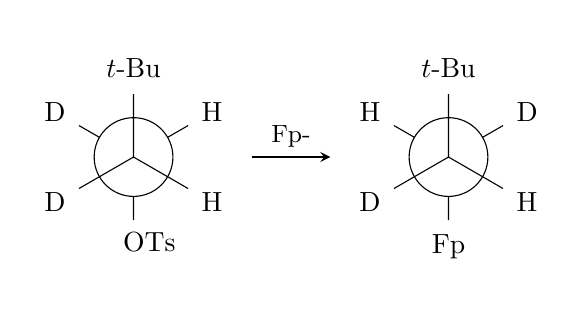
\begin{tikzpicture}[
                every node/.style={circle}
            ]
                \begin{scope}
                    \draw circle (0.5cm);
                    \draw 
                        (0,0) -- (90:0.8) node[above=-2mm]{$t$-Bu}
                        (30:0.5) -- (30:0.8) node[anchor=-150]{H}
                        (0,0) -- (-30:0.8) node[anchor=150]{H}
                        (-90:0.5) -- (-90:0.8) node[anchor=113,yshift=2mm]{OTs}
                        (0,0) -- (-150:0.8) node[anchor=30]{D}
                        (150:0.5) -- (150:0.8) node[anchor=-30]{D}
                    ;
                \end{scope}
                \draw [semithick,-stealth] (1.5,0) -- node[above=-2mm]{\small\ce{Fp-}} (2.5,0);
                \begin{scope}[xshift=4cm]
                    \draw circle (0.5cm);
                    \draw 
                        (0,0) -- (90:0.8) node[above=-2mm]{$t$-Bu}
                        (30:0.5) -- (30:0.8) node[anchor=-150]{D}
                        (0,0) -- (-30:0.8) node[anchor=150]{H}
                        (-90:0.5) -- (-90:0.8) node[below=-1mm]{Fp}
                        (0,0) -- (-150:0.8) node[anchor=30]{D}
                        (150:0.5) -- (150:0.8) node[anchor=-30]{H}
                    ;
                \end{scope}
            \end{tikzpicture}
            \caption{The reaction.}
            \label{fig:SN2-stereochemistryb}
        \end{subfigure}
        \caption{S\textsubscript{N}2 stereochemistry.}
        \label{fig:SN2-stereochemistry}
    \end{figure}
    \begin{itemize}
        \item Observes inversion (by looking at $\text{J}_{\ce{H-H}}$ coupling by NMR) of \ce{H} and \ce{D} at a single stereocenter.
        \item React the compound in Figure \ref{fig:SN2-stereochemistrya} with a \ce{Fp-} fragment.
        \item Observe inversion, as in Figure \ref{fig:SN2-stereochemistryb}, so it's S\textsubscript{N}2.
    \end{itemize}
    \item Another synthesis:
    \begin{figure}[h!]
        \centering
        \schemestart
            \chemfig{(<[:-120]D)(>:[:-160]H)(-[:120]TsO)-(<[:60]D)(>:[:20]H)-[:-60]{\emph{t}-}Bu}
            \arrow{->[{Pd\textsuperscript{0}}]}
            \chemfig{(<[:-120]H)(>:[:-160]D)(-[:120]Pd-[1]OTs)-(<[:60]D)(>:[:20]H)-[:-60]{\emph{t}-}Bu}
            \arrow{->[PhMgBr]}
            \chemfig{(<[:-120]H)(>:[:-160]D)(-[:120]Pd-[1]Ph)-(<[:60]D)(>:[:20]H)-[:-60]{\emph{t}-}Bu}
            \arrow{->[red. elim.]}
            \chemfig{(<[:-120]H)(>:[:-160]D)(-[:120]Ph)-(<[:60]D)(>:[:20]H)-[:-60]{\emph{t}-}Bu}
        \schemestop
        \caption{An additional way of probing S\textsubscript{N}2 addition/elimination.}
        \label{fig:SN2-additionalSynthesis}
    \end{figure}
    \begin{itemize}
        \item This one shows us that palladium causes an inversion once again, but reductive elimination does not.
    \end{itemize}
    \item Radical mechanisms.
    \begin{itemize}
        \item We probe these with \textbf{radical clocks}.
        \item The unzipping of the methylcyclopropane radical ring happens so fast that it will necessarily be faster than any recombination with \ce{M-Cl}.
        \item Since iodides are easier to reduce than bromides, bromomethylcyclopropane will react in a straightforward manner with \ce{Fp-}, but iodomethylcyclopropane and \ce{Fp-} will pursue a radical mechanism to a competitive degree. Why does the reduction potential of iodides and bromides matter?
    \end{itemize}
    \item \textbf{Radical clock}: A reagent such that if a radical is generated on it, it will undergo a rapid isomerization or redistribution to generate different product(s).
    \item A few notes.
    \begin{enumerate}
        \item Similar rules to those in orgo apply.
        \begin{itemize}
            \item For example, \ce{I-} is a better leaving group than \ce{Cl-}.
            \item However, there are exceptions, too: \ce{CN} is a terrible leaving group in inorganic chemistry, whereas you can sometimes kick it out in orgo.
        \end{itemize}
        \item Sterics matter.
        \begin{itemize}
            \item Oxidative addition is slower for sterically encumbered substrates.
            \item If you want to favor a radical reaction over a concerted or nucleophilic mechanism, make the compound bulky. This will disfavor the two undesired mechanisms but not an electron transfer step.
        \end{itemize}
        \item First row metals will be faster than second and third row metals.
        \begin{itemize}
            \item This is because they're much more reactive. However, they will also go down competitive side paths more readily (can be good or bad).
            \item Because of this, second and third row metals are more often used. Plus, you can just heat them up a bit to speed up the reaction.
        \end{itemize}
    \end{enumerate}
\end{itemize}



\section{Lecture 7: Insertion/Deinsertion and Kinetics}
\begin{itemize}
    \item \marginnote{4/12:}Migratory insertion/deinsertion.
    \item Also pretty unique to the transition metals.
    \item General form:
    \begin{equation*}
        \ce{L-M^Q-X <=>[{insertion}][{deinsertion}] M^Q-L-X}
    \end{equation*}
    \begin{itemize}
        \item In the course of this reaction, the \ce{L} is converted into an X-type ligand.
    \end{itemize}
    \item Characteristics of insertion: Electron count decreases by 2, coordination number decreases by 1, and the oxidation state does not change.
    \item Examples:
    \begin{itemize}
        \item 1,1-insertion: \ce{Me-M-CO <=> M-C(=O)-Me}.
        \begin{itemize}
            \item So named because the metal and the migrating group end up at the same position on the carbonyl ligand (the 1 position).
        \end{itemize}
        \item 1,2-migration: \ce{Cp2Zr(-||)Me <=> Cp2ZrPr}.
        \begin{itemize}
            \item So named because the metal ends up on the 1 position of the ethylene olefin and the migrating group ends up on the 2 position of the ethylene olefin (remember that we number substituents from the metal center outwards).
        \end{itemize}
    \end{itemize}
    \item More groups than methyl can migrate; it's just that methyl commonly migrates.
    \item Insertions into \ce{M-C} bonds are common.
    \begin{itemize}
        \item Insertions into \ce{M-H} bonds are common for olefins, but uncommon for \ce{CO} because metal carbonyl species are unstable.
        \item You can also insert into \ce{M-O} bonds (note that dppe stands for diphenylphosphinoethane):
        \begin{figure}[h!]
            \centering
            \schemestart
                \chemfig{Pt?(-[3]\chemabove{P}{Ph_2}-[:-150]-[6,0.9]-[:-30]\chembelow{P}{Ph_2}?)(-[7]Me)(-[1]OMe)}
                \arrow(.east--.-173){->[CO]}
                \chemfig{{(dppe)}Pt(-[7]Me)(-[:30](=[2,0.7]O)-[:-30]OMe)}
            \schemestop
            \vspace{1em}
            \caption{Insertion into an \ce{M-O} bond.}
            \label{fig:insertion-M-O}
        \end{figure}
    \end{itemize}
    \item A note on the mechanism:
    \begin{itemize}
        \item We can either take the perspective that the X group migrates or that the L group inserts itself into the \ce{M-X} bond.
        \item Thus, either the $\sigma$ bond of the migrating ligand attacks the site to which it bonds or the L group moves into the $\sigma$ bond.
        \item We call this a migratory insertion, but there are two possible mechanisms (it's hard to know what is migrating and what is staying put).
        \item Answer: The X-type ligand is migrating. We can test this by radiolabeling one of the carbonyls in \ce{Mn(CO)5Me}?
    \end{itemize}
    \item $\beta$-\ce{H} elimination: \ce{L2NiEt <=> L2Ni(-||)H}.
    \begin{figure}[H]
        \centering
        \chemleft{[}
            \chemfig{\charge{-30=\:}{Ni}?-[1]-[:-30]-[:-110]H?[,,dashed]}
        \chemright{]^\ddagger}
        \caption{The transition state in a $\beta$-\ce{H} elimination.}
        \label{fig:betaHydrideTransState}
    \end{figure}
    \begin{itemize}
        \item The transition state (see Figure \ref{fig:betaHydrideTransState}) shows an \textbf{agostic interaction}.
    \end{itemize}
    \item $\alpha$-elimination.
    \begin{figure}[H]
        \centering
        \schemestart
            \chemfig{Pt?(-[3]\chemabove{P}{R_2}-[:-150]-[6,0.9]-[:-30]\chembelow{P}{R_2}?)(-[1]SiAr_2(-[:120,0.7,1]H))(-[7]Me)}
            \+
            \chemfig{B{(C_6F_5)_3}}
            \arrow(.-7--.west){->[][\small{-MeB(ArF)\textsubscript{3}\textsuperscript{--}}]}[0,1.5]
            \chemleft{[}
                \chemfig{\charge{120[yshift=1mm]=$\oplus$}{Pt}?-[1]\chemabove{Si}{Ar_2}-[7]H?[,,dashed]}
            \chemright{]^\ddagger}
            \arrow
            \chemleft{[}
                \chemfig{Pt?(-[3]\chemabove{P}{R_2}-[:-150]-[6,0.9]-[:-30]\chembelow{P}{R_2}?)(-[7]H)(=[1]SiAr_2)}
            \chemright{]^+}
        \schemestop
        \caption{An example of $\alpha$-elimination.}
        \label{fig:alphaElimination}
    \end{figure}
    \item External attack at a ligand.
    \begin{figure}[H]
        \centering
        \ce{L_nM^Q=X + Nu- <=> [L_nM^{Q-2}-X-Nu]-}\\[1em]
        \schemestart
            \chemfig{L_{\emph{n}}M^{\emph{Q}}-\phantom{i}-[6,0.3]Y=[2]X}
            \arrow{->[Nu\textsuperscript{--}]}
            \chemleft{[}
                \chemfig{L_{\emph{n}}M^{\emph{Q}}-[:30]X-[:-30]Y-[:30]Nu}
            \chemright{]^-}
        \schemestop\\[1em]
        \schemestart
            \chemfig{L_{\emph{n}}M^{\emph{Q}}-X~Y}
            \arrow{->[Nu\textsuperscript{--}]}
            \chemleft{[}
                \chemfig{L_{\emph{n}}M^{\emph{Q}}-[:30]X(=[2]Y)-[:-30]Nu}
            \chemright{]^-}
        \schemestop
        \caption{Types of external attack at a ligand.}
        \label{fig:externalLigandAttack}
    \end{figure}
    \begin{itemize}
        \item Somewhat more related to organic chemistry.
        \item Lists some examples.
    \end{itemize}
    \item \ce{Tp} is trispyrazolylborate.
    \begin{itemize}
        \item It's a \ce{Cp} analogue, meaning that it has the same electron count and similar sterics.
    \end{itemize}
    \item Be aware of Fischer carbenes.
    \item There could be a radical process.
    \begin{itemize}
        \item \textcite{bib:CrevierMayer} tells us that an osmium-nitrido external attack at a ligand must be a 2-electron process, not a radical mechanism.
    \end{itemize}
    \item Electrophilic attack on a ligand.
    \item Example: \ce{Ir^{II}(PPh3)2HCl(NO) ->[HCl] Ir^{III}(PPh3)2HCl2(N(=O)H)}.
    \begin{itemize}
        \item The reactant is a $16\,\e[-]$ species.
        \item The nitrogen-containing ligand is a nitroxyl ligand.
    \end{itemize}
    \item Gives some other examples.
    \item \ce{Tp^*} is a \ce{Tp} group where each pyrazole is 3,5-dimethyl substituted.
    \item Sometimes we create a positive metal cation. This can be accomplished either via a direct electrophilic attack on an attached R group or via an attack at the metal followed by reductive elimination.
    \item $\sigma$-bond metathesis: \ce{L_nM^Q-X + Y-Z <=> L_nM^Q-Y + X-Z}.
    \begin{itemize}
        \item Usually observed for $d^0$ systems.
    \end{itemize}
    \item Example: \ce{Zr^{IV}(N(SiR3)H)3Me -> Zr(N(SiR3)H)2(=N-SiR3) + CH4}.
    \begin{itemize}
        \item \ce{C-H} activation is a big thing in synthetic chemistry, and a lot of the pathways go through $d^0$, early, reactive transition metals.
    \end{itemize}
    \item More on $\sigma$-bond metathesis:
    \begin{enumerate}
        \item Most common for early metals.
        \begin{itemize}
            \item Especially $d^0$ metals.
        \end{itemize}
        \item Thought to go through a 4-membered transition state.
        \item There is likely a continuum between "pure" $\sigma$-bond metathesis and oxidative addition/reductive elimination.
        \item This still requires an open coordination site and $\leq 16\,\e[-]$.
        \begin{itemize}
            \item Because the first step is coordination, usually to form some kind of $\sigma$-adduct.
        \end{itemize}
    \end{enumerate}
    \item Kinetics of associative substitution.
    \begin{equation*}
        \text{rate} = -\dv{\ce{[ML_x]}}{t}
        = \dv{\ce{[ML_{x-1}L$'$]}}{t}
        = k\ce{[ML_x][L$'$]}
    \end{equation*}
    \begin{figure}[h!]
        \centering
        \begin{subfigure}[b]{0.45\linewidth}
            \centering
            \begin{tikzpicture}[
                every node/.style={black}
            ]
                \small
                \draw (5,0) -- (0,0) -- node[left]{$\ln\ce{[ML_x]}$} (0,4);
                \footnotesize
                \draw (2,0.1) -- ++(0,-0.2) node[below]{$t_{1/2}$};
    
                \draw [blx,thick] (0.2,3.7) -- (4.3,0.5);
                \draw [grx,thick] (0.2,3.5) -- (1.9,0.2) node[above right,yshift=-1mm]{high \ce{[L$'$]}};
                \draw [rex,thick] (0.35,3.7) -- (4.3,2.5) node[below]{Low \ce{[L$'$]}};
            \end{tikzpicture}
            \caption{Reaction coordinate and \ce{[ML_x]}.}
            \label{fig:associativeKineticsa}
        \end{subfigure}
        \begin{subfigure}[b]{0.45\linewidth}
            \centering
            \begin{tikzpicture}[
                every node/.style={black}
            ]
                \small
                \draw (5,0) -- node[below]{\ce{[L$'$]}} (0,0) -- node[left]{$k_\text{obs}$} (0,4);
                \footnotesize
    
                \draw [blx,thick] (0.2,0.2) -- (4,3.4) node[below right,yshift=1mm]{Theory};
                \draw [grx,thick] (0.2,0.2) to[out=52,in=-140] (4,3.8) node[above right,yshift=-1mm]{Experiment};
            \end{tikzpicture}
            \caption{Rate and \ce{[L$'$]}.}
            \label{fig:associativeKineticsb}
        \end{subfigure}
        \caption{Kinetics of associative substitution.}
        \label{fig:associativeKinetics}
    \end{figure}
    \begin{itemize}
        \item Experimentally, we can use a large \ce{[L$'$]} to get to pseudo-first order conditions.
        \item This gives us $\text{rate}=k_\text{obs}\ce{[ML_x]}$ where $k_\text{obs}=k\ce{[L$'$]}$.
        \item In Figure \ref{fig:associativeKineticsa}, $t_{1/2}$ is a midpoint, and the rate gets faster (steeper slope) with more \ce{[L$'$]} and slower (more gradual slope) with less \ce{[L$'$]}.
        \item There is a discrepancy between theory and experiment in Figure \ref{fig:associativeKineticsb}.
        \begin{itemize}
            \item This is because of the presence of a solvent-assisted mechanism.
            \item \ce{L_xM + {solv} <=>[$k_s$] L_{x-1}ML({solv}) ->[L$'$][{fast}] L_{x-1}ML$'$ + {solv} + L}.
            \item Note that $k_s$ is the rate of solvent association.
        \end{itemize}
        \item The solvent-assisted mechanism dominates at low \ce{[L$'$]}, and vice versa for the normal mechanism.
    \end{itemize}
    \item Kinetics of dissociative substitutions.
    \begin{enumerate}[label={\roman*)}]
        \item \ce{ML_x <=>[$k_1$][$k_{-1}$] [ML_{x-1}] + L}.
        \item \ce{[ML_{x-1}] + L$'$ ->[$k_2$] ML_{x-1}L$'$} (assume irreversible).
    \end{enumerate}
    \begin{itemize}
        \item There are now two cases:
        \begin{enumerate}[label={\alph*)}]
            \item Fast pre-equilibrium, i.e., $k_1,k_{-1}>>k_2$. This gives us
            \begin{equation*}
                \text{rate} = k_1k_2\cdot\frac{\ce{[ML_x][L$'$]}}{\ce{[L]}}
            \end{equation*}
            \item Steady state approximation: $
                \dv*{\ce{[ML_{x-1}]}}{t} = 0
                = k_1\ce{[ML_x]}-k_{-1}\ce{[ML_{x-1}]}-k_2\ce{[ML_{x-1}][L$'$]}
            $. If we solve the above for \ce{[ML_{x-1}]}, then we get
            \begin{equation*}
                \text{rate} = \frac{k_1k_2\ce{[ML_x][L$'$]}}{k_{-1}\ce{[L]}+k_2\ce{[L$'$]}}
            \end{equation*}
            If we now assume that $k_2\ce{[L$'$]}$ is large, then we get $\text{rate}=k_1\ce{[ML_x]}$.
            \begin{itemize}
                \item The steady state approximation is a good assumption to make because if you see a buildup of the dissociative intermediate, you can measure the rates. Alternatively, if you don't see it, you can assume that $\ce{[ML_{x-1}]}=0$.
            \end{itemize}
        \end{enumerate}
        \item To do this experimentally, we add a large concentration of \ce{[L$'$]}, or \ce{[L]} in some cases.
        \begin{itemize}
            \item This gives us $\text{rate}=k_\text{obs}\ce{[ML_x]}$ where $k_\text{obs}$ denotes the mess from the above equation.
        \end{itemize}
        \begin{figure}[h!]
            \centering
            \begin{tikzpicture}
                \small
                \draw (5,0) -- node[below]{\ce{[L$'$]}} (0,0) -- node[left]{$k_\text{obs}$} (0,4);
                \footnotesize
        
                \draw [semithick,dashed] (0,2.5) -- (4.5,2.5);
                \draw [blx,thick] (0,0) to[out=60,in=-175] (4.5,2.3);
        
                \node [anchor=south west] at (1.3,0.1) {2nd order region}
                    edge [->,out=180,in=-60] (0.7,0.8)
                ;
                \node [anchor=south east] at (3.5,2.6) {1st order region}
                    edge [->,out=0,in=120] (4,2.35)
                ;
            \end{tikzpicture}
            \caption{The effect of \ce{[L$'$]} on rate.}
            \label{fig:LPrimeRate}
        \end{figure}
        \item If we plot $k_\text{obs}$ vs. \ce{[L$'$]}, we get Figure \ref{fig:LPrimeRate}.
        \begin{itemize}
            \item In the second order region, \ce{ML_x <=>[{fast}] ML_{x-1}} many times before product formation.
            \item In the first order region, every time \ce{ML_{x-1}} forms, it goes on to become a product.
        \end{itemize}
        \item In other words, $k_\text{obs}$ should approach $k_1$ when $k_2\ce{[L$'$]}>>k_{-1}\ce{[L]}$.
        \item Importantly, as \ce{L$'$} is varied with different ligands, $k_1$ should stay constant (assuming the mechanism doesn't change).
        \item A double reciprocal plot can be used to obtain still more information about the reaction.
        \begin{itemize}
            \item If you plot $\frac{1}{k_\text{obs}}$ vs. $\frac{\ce{[L]}}{\ce{[L$'$]}}$ and run a linear regression, the slope will be $\frac{k_{-1}}{k_1k_2}$ and the $y$-intercept will be $\frac{1}{k_1}$.
        \end{itemize}
    \end{itemize}
    \item Transition state theory basics:
    \begin{itemize}
        \item In 1887, Arrhenius comes up with the Arrhenius equation $k=A\e[-E_A/RT]$, which can be algebraically manipulated into
        \begin{equation*}
            \ln k = \ln A-\frac{E_A}{RT}
        \end{equation*}
        where $E_A$ is the activation energy, $R$ is the gas constant, and $T$ is temperature.
        \begin{itemize}
            \item This allows us to create a linear $\ln k$ vs. $\frac{1}{T}$ plot from which we can pull out important information.
        \end{itemize}
        \item In the 1930s, Eyring comes up with the Eyring equation
        \begin{equation*}
            \ln\left( \frac{k}{T} \right) = \frac{-\Delta H^\ddagger}{RT}+\ln\left( \frac{k_B}{h} \right)+\frac{\Delta S^\ddagger}{R}
        \end{equation*}
        where we can calculate that $\ln(k_B/h)\approx 23.76$.
        \begin{itemize}
            \item This allows us to create a linear $\ln(k/T)$ vs. $\frac{1}{T}$ plot from which we can pull out additional important information.
        \end{itemize}
    \end{itemize}
\end{itemize}




\end{document}